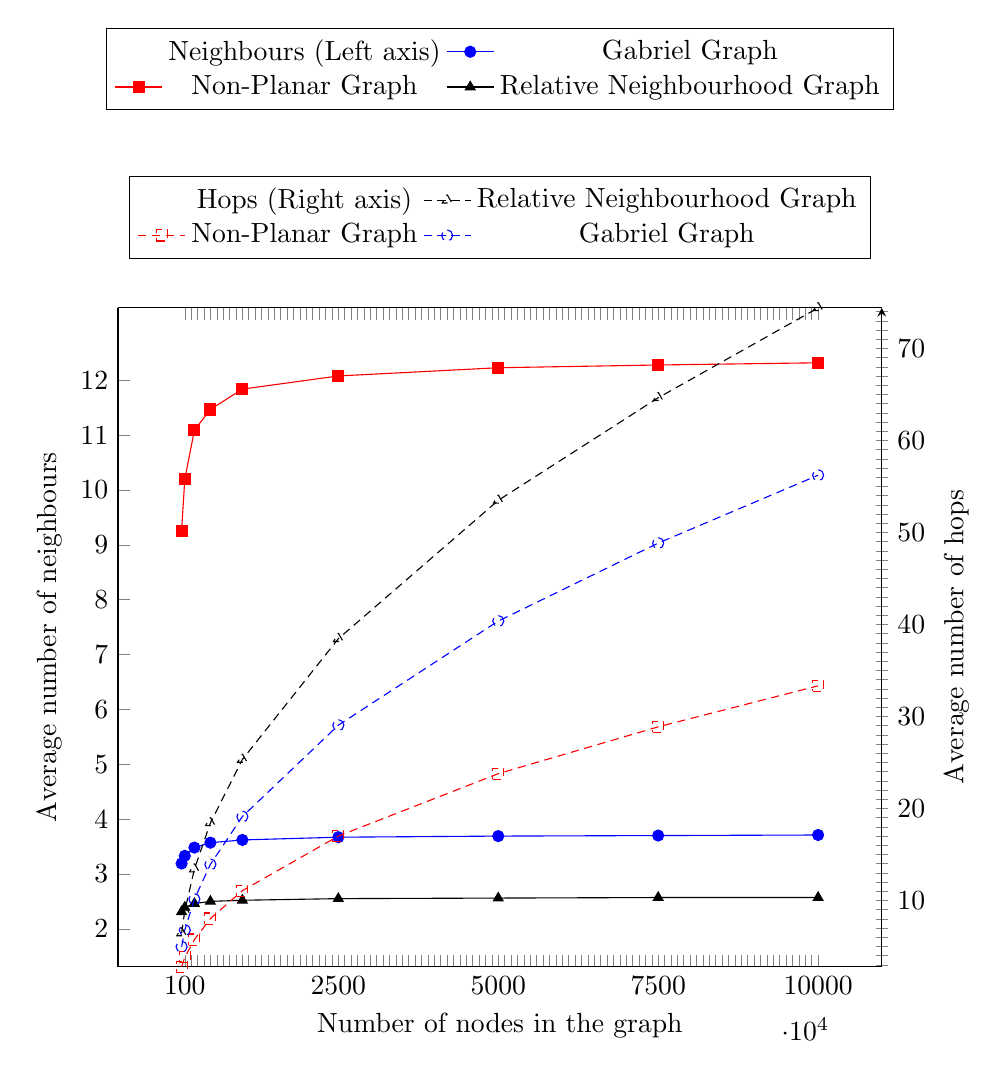
\begin{tikzpicture}
\pgfplotsset{every axis legend/.append style={at={(0.5,1.30)},anchor=south}}
\begin{axis}[scale only axis, xtick={100, 200, 300, 400, 500, 600, 700, 800, 900, 1000, 1100, 1200, 1300, 1400, 1500, 1600, 1700, 1800, 1900, 2000, 2100, 2200, 2300, 2400, 2500, 2600, 2700, 2800, 2900, 3000, 3100, 3200, 3300, 3400, 3500, 3600, 3700, 3800, 3900, 4000, 4100, 4200, 4300, 4400, 4500, 4600, 4700, 4800, 4900, 5000, 5100, 5200, 5300, 5400, 5500, 5600, 5700, 5800, 5900, 6000, 6100, 6200, 6300, 6400, 6500, 6600, 6700, 6800, 6900, 7000, 7100, 7200, 7300, 7400, 7500, 7600, 7700, 7800, 7900, 8000, 8100, 8200, 8300, 8400, 8500, 8600, 8700, 8800, 8900, 9000, 9100, 9200, 9300, 9400, 9500, 9600, 9700, 9800, 9900, 10000}, xticklabels={$100$, , , , , , , , , , , , , , , , , , , , , , , , $2500$, , , , , , , , , , , , , , , , , , , , , , , , , $5000$, , , , , , , , , , , , , , , , , , , , , , , , , $7500$, , , , , , , , , , , , , , , , , , , , , , , , , $10000$}, ytick={1,...,12}, yticklabels={1,...,12}, transpose legend, legend columns=2, width=0.8\linewidth, axis y line*=left, xlabel=Number of nodes in the graph, ylabel=Average number of neighbours]
\addlegendimage{legend image code/.code=}
\addlegendentry{Neighbours (Left axis)}
\addplot[color=red, mark=square*] coordinates{
	(50, 9.26)
	(100, 10.20)
	(250, 11.09)
	(500, 11.47)
	(1000, 11.84)
	(2500, 12.08)
	(5000, 12.23)
	(7500, 12.28)
	(10000, 12.32)
}; \addlegendentry{Non-Planar Graph}
\addplot[color=blue, mark=*] coordinates{
	(50, 3.19)
	(100, 3.33)
	(250, 3.48)
	(500, 3.57)
	(1000, 3.62)
	(2500, 3.67)
	(5000, 3.69)
	(7500, 3.70)
	(10000, 3.71)
}; \addlegendentry{Gabriel Graph}
\addplot[color=black, mark=triangle*] coordinates{
	(50, 2.31)
	(100, 2.39)
	(250, 2.46)
	(500, 2.50)
	(1000, 2.52)
	(2500, 2.55)
	(5000, 2.56)
	(7500, 2.57)
	(10000, 2.57)
}; \addlegendentry{Relative Neighbourhood Graph}
\end{axis}

\pgfplotsset{every axis legend/.append style={at={(0.5,1.2)},anchor=north}}
\begin{axis}[scale only axis, ytick={1, 2, 3, 4, 5, 6, 7, 8, 9, 10, 11, 12, 13, 14, 15, 16, 17, 18, 19, 20, 21, 22, 23, 24, 25, 26, 27, 28, 29, 30, 31, 32, 33, 34, 35, 36, 37, 38, 39, 40, 41, 42, 43, 44, 45, 46, 47, 48, 49, 50, 51, 52, 53, 54, 55, 56, 57, 58, 59, 60, 61, 62, 63, 64, 65, 66, 67, 68, 69, 70, 71, 72, 73, 74, 75, 76, 77, 78, 79, 80, 81, 82, 83, 84, 85, 86, 87, 88, 89, 90, 91, 92, 93, 94, 95, 96, 97, 98, 99, 100}, yticklabels={, , , , , , , , , $10$, , , , , , , , , , $20$, , , , , , , , , , $30$, , , , , , , , , , $40$, , , , , , , , , , $50$, , , , , , , , , , $60$, , , , , , , , , , $70$, , , , , , , , , , $80$, , , , , , , , , , $90$, , , , , , , , , , $100$}, width=0.8\linewidth, transpose legend, legend columns=3, axis y line=right, axis x line=none, ylabel=Average number of hops]
\addlegendimage{legend image code/.code=}
\addlegendentry{Hops (Right axis)}
\addplot[color=red, mark=square, densely dashed] coordinates{
	(50, 2.80)
	(100, 3.81)
	(250, 5.75)
	(500, 8.03)
	(1000, 11.06)
	(2500, 17.00)
	(5000, 23.78)
	(7500, 28.87)
	(10000, 33.33)
}; \addlegendentry{Non-Planar Graph}
\addplot[color=blue, mark=o, densely dashed] coordinates{
	(50, 4.97)
	(100, 6.78)
	(250, 10.14)
	(500, 13.92)
	(1000, 19.12)
	(2500, 29.05)
	(5000, 40.37)
	(7500, 48.84)
	(10000, 56.22)
}; \addlegendentry{Gabriel Graph}
\addplot[color=black, mark=triangle, densely dashed] coordinates{
	(50, 6.46)
	(100, 8.87)
	(250, 13.41)
	(500, 18.43)
	(1000, 25.32)
	(2500, 38.45)
	(5000, 53.49)
	(7500, 64.64)
	(10000, 74.41)
}; \addlegendentry{Relative Neighbourhood Graph}
\end{axis}
\end{tikzpicture}
